\section{Systemanalyse}
\begin{frame}{Hændelsestabel}
	\framesubtitle{}
	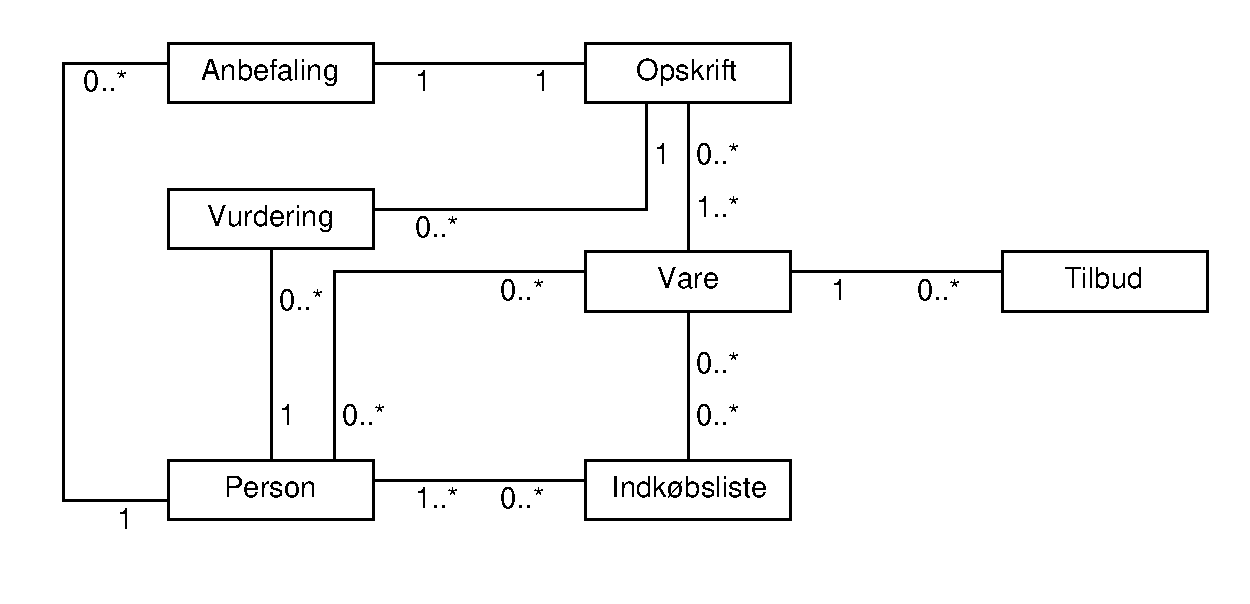
\includegraphics[width=1\textwidth]{images/klassediagram_model_simple.pdf}
\end{frame}
\begin{frame}{Klassediagram over problemområdet}
	\framesubtitle{}
	\begin{table}[h]
  \centering
    \colorlet{shadecolor}{gray!40}
    \rowcolors{1}{white}{shadecolor}
    \scalebox{0.7}{
      \begin{tabular}{l|lccccccc}
      %\hline
       								& \rot{Tilbud}  & \rot{Indkøbsliste} & \rot{Opskrift} & \rot{Vare} & \rot{Person}& \rot{Vurderinger} \\ \hline
      Vare tilføjet til indkøbsliste&               & *      &          & *     &       &   \\
      Vare fjernet fra indkøbsliste	&              	& *      &          & *     &       &   \\
      Vare aftjekket på indkøbsliste&               & *      &          & *     &       &   \\
      \rowcolor{black!30}
      Tilbud oprettet        		& +            	&        &          & *     &       &   \\
      Tilbud aktiveret        		& +            	&        &          & *     &       &   \\
      Tilbud udgået          		& +        		&        &      	& *     &       &   \\
      Vare tilføjet til overvågning &           	&        &          & *     &       &   \\
      Vare fjernet fra overvågning  &           	&        &          & *     &       &   \\
      Overvågningsvare på tilbud    & *  			&		 &			& * 	& *		&	\\
      Del indkøbsliste       		&               & *      &          &       & *     &   \\
      Indkøbsliste oprettet  		&              	& +      &          &       & *     &   \\
      Indkøbsliste slettet  		&             	& +      &          &       & *     &   \\
      Forlad Indkøbsliste			&				& *		 & 			&		& *		&   \\
      Opskrift oprettet				&				&		 & +		& *  	& *		& 	\\
      Opskrift slettet				&				&		 & +		& *  	& *		& 	\\
      Opskrift klonet				&				&		 & *		& *		& *		&	\\			
      Vurdering givet				&             	&        & *        &       & *		& * \\
      Anbefaling givet				&				&		 & *		&		& *		& * \\

    \end{tabular}
  }
\end{table}

\end{frame}
\begin{frame}{Funktioner}
	\framesubtitle{Hvad kunne tilføjes?}
	\begin{table}[h]
  \centering
  %\tiny
   	\colorlet{shadecolor}{gray!40}
    \rowcolors{1}{white}{shadecolor}
    \scalebox{0.64}{
      \begin{tabular}{l|lllll}
      %\hline
      \textbf{Funktioner}			& {Kompleksitet}	& {Kategori}  	\\ \hline
      Log ind						& Medium			& Beregning, Opdatering		\\
      Log ud						    & Simpel			& Opdatering	\\
      Registrer bruger				& Simpel			& Opdatering	\\
      Tilføje varer til lister		& Simpel       & Opdatering	\\
      Fjerne varer fra lister		& Simpel       		& Opdatering	\\
      Oprette og slette indkøbslister & Simpel       	& Opdatering	\\
      Forlad indkøbsliste			& Simpel			& Opdatering \\
      Dele Indkøbsliste				& Medium       		& Opdatering	\\
      Søgning på tilbud for varer    & Medium     		& Beregning		\\
      Sætte præferencer				& Simpel       		& Opdatering	\\
      Filtrere for præferencer		& Kompleks     		& Beregning		\\
      Give vurdering				& Simpel       		& Opdatering	\\
      Sende anbefaling				& Meget kompleks	& Aflæsning, signalering, beregning		\\
      Meddele tilbud på varer		& Medium      		& Signalering	\\
	  Se opskrifter					& Simpel       		& Aflæsning		\\
      Oprette opskrift      		& Simpel            & Opdatering  	\\
      Ændre opskrift        		& Simpel            & Opdatering	\\
      Klone	opskrift       			& Simpel            & Opdatering 	\\
      Slette opskrift				& Simpel			& Opdatering	\\
      Skaler opskrift				& Simpel			& Beregning		\\
	  Se tilbud						& Simpel       		& Aflæsning		\\
      Hente tilbud					& Simpel	       	& Opdatering	\\
    \end{tabular}
	}
  %\caption{\tiny Funktionstabel. Viser de forskellige funktioner der skal bruges, samt deres kompleksitet og kategori.}\label{tabel:functionstable}
  
\end{table}
\end{frame}

\begin{frame}{Kravspecifikation}
	\framesubtitle{Hvad bruger vi det til?}
	\begin{itemize} 
    	\item Userstories
    	\begin{itemize}
    		\item SCRUM
    	\end{itemize}
    	\item Klar oversigt over hvad der skal laves
    	\item Forsåelse af problem- og anvendelsesområde
  	\end{itemize}
    \begin{beamerboxesrounded}[upper=headerCol,lower=bodyCol,shadow=true]{Exempel på userstorie}
    \textit{Som en bruger vil jeg kunne overvåge specifikke varer og få en notifikation, når disse
varer kommer på tilbud.}
    \end{beamerboxesrounded}

\end{frame}
\begin{frame}{Manglende materiale fra OOA\&D}
	\framesubtitle{Udokumenteret brug af modeller}
	\begin{itemize} 
    \item Adfærdsmønstre
    \item 
    \item 
  \end{itemize}
\end{frame}